
\paragraph{MOT Challenge Format}

{
    To make the collected data useful for the tracking system, it must undergo a labeling process. 
    The main annotation format that was used is the \textbf{\ac{MOT} Challenge format}\cite{MOTChallenge2015}, 
    which is well-suited for both object tracking and object detection in videos. 
    This format is implemented as a \ac{CSV} text file per video with each line containing 10 fields: 
}

\begin{center}
    {``Frame, Id, left, top, width, height, confidence, 3D-World x, 3D-World y, 3D-World z"}
\end{center}

{
    In the case of 2D data, the 3D-World values are set to -1 and, in the case of detections, the Id value is also set to -1.
}

%\begin{table}[!h]
%    \centering
%    \caption[MOT Challenge format]{ \footnotesize MOT Challenge format with default values.}
%    \label{tab:MOT Challenge format}
%
%    \begin{tabularx}{\textwidth}{@{\hspace{1em}}Xl@{\hspace{1em}}|@{\hspace{1em}}X@{\hspace{1em}}X@{\hspace{1em}}}
%        \toprule
%        \textbf{Column} & \textbf{Field Name} & \textbf{Detection} & \textbf{Tracking} \\
%        \midrule
%        \midrule
%        1 & Frame number & \textless frame\textgreater & \textless frame\textgreater \\
%        2 & Identity number & -1 & \textless id\textgreater \\
%        3 & Detection left & \textless bb\_left\textgreater & \textless bb\_left\textgreater \\
%        4 & Detection top & \textless bb\_top\textgreater & \textless bb\_top\textgreater \\
%        5 & Detection width & \textless bb\_width\textgreater & \textless bb\_width\textgreater \\
%        6 & Detection height & \textless bb\_height\textgreater & \textless bb\_height\textgreater \\ 
%        7 & Detection confidence & \textless conf\textgreater & \textless conf\textgreater \\
%        8 & 3D World x & -1 & -1 \\
%        9 & 3D World y & -1 & -1 \\
%        10 & 3D World z & -1 & -1 \\
%        \bottomrule
%    \end{tabularx}
%
%\end{table}


{
    In addition to the main \ac{MOT} format, this project employs various dataset formats to simplify the training and deployment of different models. 
    These formats include the \ac{YOLO} dataset format\cite{yoloFormat} for image object detection, 
    the Market-1501 dataset format\cite{Market-1501} for appearance modeling, 
    and a custom format tailored for segmenting valid frames and IDs from the appearance videos.
}

\paragraph{YOLO Format}

{
    The \ac{YOLO} format is utilized for labeling single images extracted from videos. 
    Each image is associated with an equally named \ac{CSV} text-file that contains the following column fields for each detection:
}

\begin{center}
    {``class id, x-axis center, y-axis center, width, height"}
\end{center}

{
    It's important to note that the image fields are normalized based on the image shape. 
    Additionally, the \ac{YOLO} format defines a specific folder structure that separates images and labels into subfolders stemming from the same root. 
    A YAML file is used to describe the data paths and class indexes for each dataset.
}

{
    A tool was developed to convert the videos with a MOT Challenge annotations into images with a valid \ac{YOLO} format dataset. 
    This tool offers the flexibility to crop images (and the corresponding labels) into different segments, ensuring that each segment contains at least one whole ant in a random position. 
    The cropping feature maximizing the number of whole ants within each crop while guaranteeing that each ant is fully visible in at least one crop.
    Figure \ref{fig:yolo crop} shows an example of the results of this tool on a video.
}

\begin{figure}[!b]
    \centering
    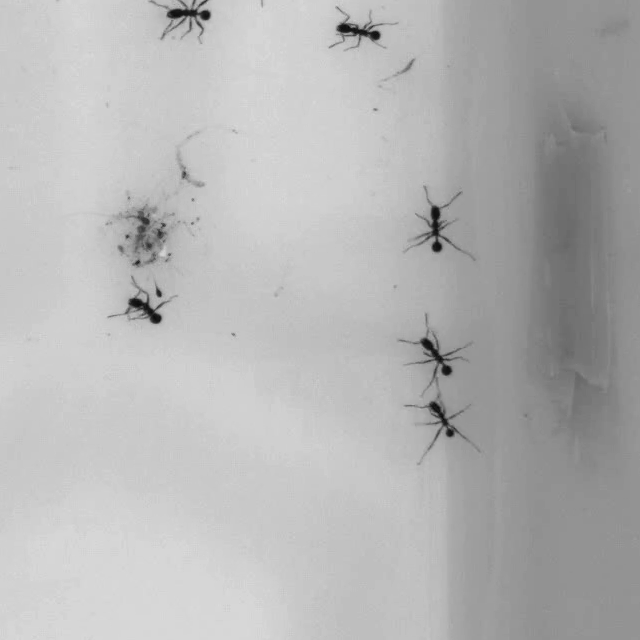
\includegraphics[width=0.4\linewidth]{figures/05_methodology/yolo_crop.png}
    \caption[YOLO dataset: crop of 640x640 px]{\footnotesize{A crop of 640x640 px generated from an annotated video to create a YOLO Dataset.}}
    \label{fig:yolo crop}
    \vspace{-3em}
\end{figure}

\FloatBarrier

\begin{figure}[!htp]
    \centering
    \begin{subfigure}[b]{0.4\linewidth}
        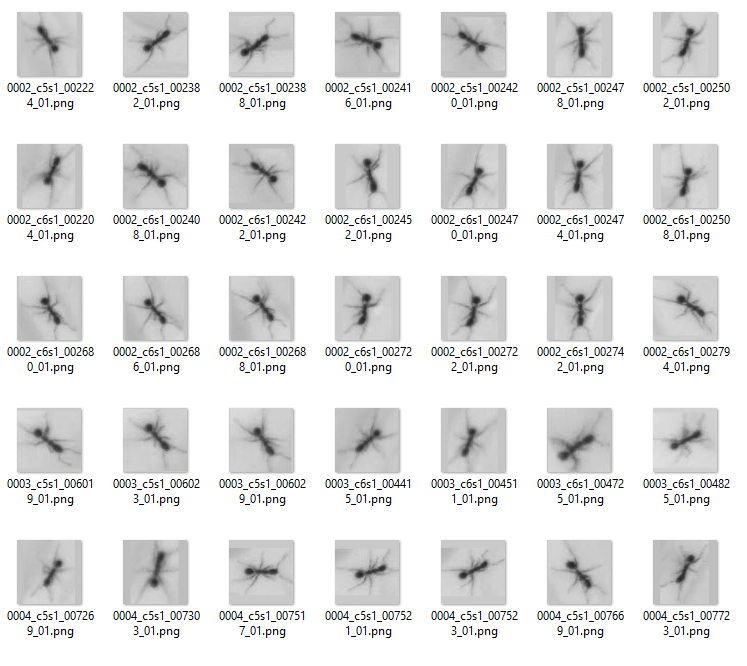
\includegraphics[width=\linewidth]{figures/05_methodology/Market_unoriented.png}
        \caption[Samples of the unoriented appearance dataset]{\footnotesize{35 samples of the unoriented appearance dataset.}}
        \label{fig:unoriented appearance}
    \end{subfigure}
    \hspace{0.025\linewidth}
    \begin{subfigure}[b]{0.4\linewidth}
        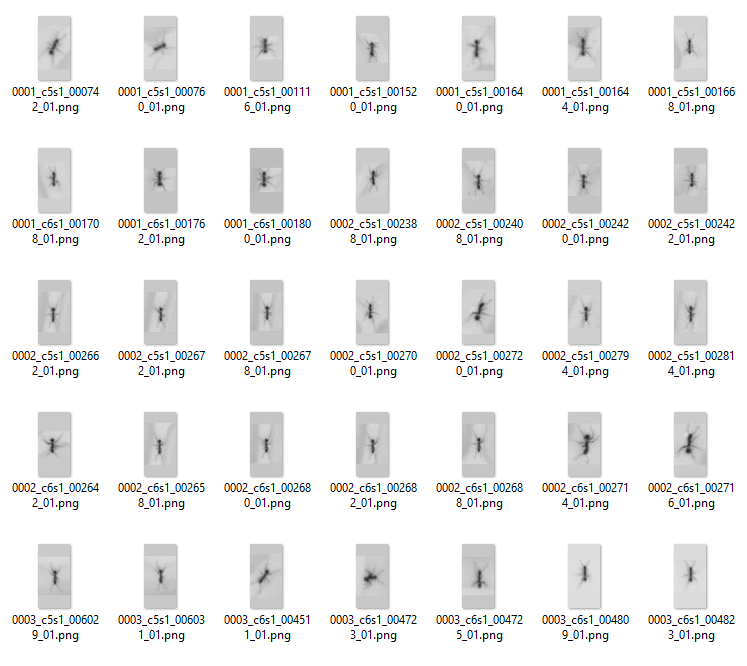
\includegraphics[width=\linewidth]{figures/05_methodology/Market_oriented.png}
        \caption[Samples of the oriented appearance dataset]{\footnotesize{35 samples of the oriented appearance dataset.}}
        \label{fig:oriented appearance}
    \end{subfigure}
    \caption[Samples of the appearance datasets]{\footnotesize{Comparison between the output of the oriented and unoriented versions of the appearance dataset generation tools.}}
    \label{fig:appearance dataset}
    \vspace{-1.5em}
\end{figure}

\paragraph{Market-1501 Format}

{
    Market-1501 is a widely-used reidentification dataset organized based on folder and filename structures. 
    In this project, we mimic this format to simplify the deployment of the appearance model training, we call it Market-1501 Format.
}

{
    In Market-1501 Format, each ``ground truth detection" is cropped from the video and saved as an image within one of three folders: train, test, or test query. 
    and contains its identity on the filename. The identity of each detection is encoded in the filename.
}

{
    To convert the videos with MOT Challenge annotations into a Market-1501 dataset, a pair of tools were developed. 
    The first tool generates square crops using one of three strategies: 
    ``cropping and padding", ``cropping, padding the small size, and reshaping", or ``cropping and reshaping".
    The second tool generates rectangular crops with the head of the ant pointing downwards; 
    the shape of the crop is adjusted using similar methods to those employed by the first tool, 
    with the "padding the small size" option in the second tool being replaced by "padding to obtain the correct aspect ratio."
}

{
    The process of orienting the head of the ant downwards involves four steps:
}

\enlargethispage{1.5\baselineskip}

\begin{enumerate}
    \item The segmentation of the cropped ant by thresholding\footnote{Thresholding (neologism): Act of splitting a set of values using a threshold value.} the luminance level of the image.
    \item The computation of the direction of the body of the ant through principal component analysis.
    \item Determining the movement direction of the ant by comparing the current frame position with the nearest frame were the ants appears (if it is a previous frame, the origin point is the previous frame).
    \item Selecting the body direction of the ant that minimize the angular difference with the movement direction.
\end{enumerate}

\needspace{0.2\textheight}

{
    Figure \ref{fig:appearance dataset} provides an example of the output from each tool. 
    In both cases, padding was applied to one side before reshaping the crop.
    While there is an improvement, it's worth noting that the orientation solution in Figure \ref{fig:oriented appearance} has some limitations, 
    with a total of 35 instances, including 17 correct cases, 15 upside-down cases, and 3 instances with incorrect orientation.
}

\FloatBarrier

\paragraph{Custom Format}

{
    The custom format for segmenting video fragments is structured as a \ac{TSV} file with three columns. 
    The first column indicates the initial frame number, 
    the second column indicates the final frame number, 
    and the last column comprises a Python-styled list of lists that represents the invalid intervals. 
    These intervals are encoded by specifying their initial and final frames.
}

{
    Labeling is a time-consuming task that necessitates human supervision. 
    To reduce the time required, we employed an existing application and developed three additional tools.  
    The research on data annotation was conducted concurrently with the creation of a tutorial designed to guide the annotation of new training videos, which was one of the project's objectives.
}

\needspace{0.2\textheight}

\subsubsection{CVAT}

{
    \ac{CVAT}\cite{cvat} is an interactive annotation tool designed for computer vision applications. 
    It provides support for importing and exporting annotations in various popular formats. 
    In this project, we primarily relied on tracking results for labeling to save time on the annotation process.
}

{
    To set up \ac{CVAT}, it should be installed as a server through their Docker image and accessed through any web browser. 
    Figure \ref{fig:CVAT} shows the annotation interface.
}

{
    \ac{CVAT} manage each id as a class. 
    Within a frame, it offers functionalities to create, delete, and modify detections. 
    Additionally, any track can be created, deleted, marked as finished, split, merged, or have its identity changed.
    For unfinished tracks with gaps in the annotations, \ac{CVAT} employs linear interpolation, which can be adjusted manually in the desired frames.
}

{
    One limitation of \ac{CVAT} is that it supports a maximum resolution of 3000x2000 pixels.  
    To work around this, we utilized ffmpeg\cite{tomar2006converting} to downsample the video file and developed two scripts to adapt the annotations accordingly. 
    The commands in Listing \ref{lst:cvat_input} are used to generate the input video and importable annotations.
}

\begin{footnotesize}
    \begin{bashcode}[float=h, label={lst:cvat_input}, language=bash, caption={Commands to obtain the CVAT compatible data}]
        ffmpeg -y -i input.mp4 -vf scale=2000:-2,setsar=1:1 -c:v libx264 "input_downsampled.mp4"
        python3 minimum_id.py input_1.txt input_2.txt
        python3 prde_to_cvat.py input_2.txt output.zip
    \end{bashcode}
\end{footnotesize}

{
    A script was also created to convert manually corrected but downsampled annotations into the desired resolution.
}

{
    Despite the availability of preannotations from tracking models and the utility of this tool, 
    annotating 1375 frames (equivalent to approximately 1 hour and 30 minutes of video) still requires around 2 hours.
}

\begin{figure}[!tp]
    \centering
    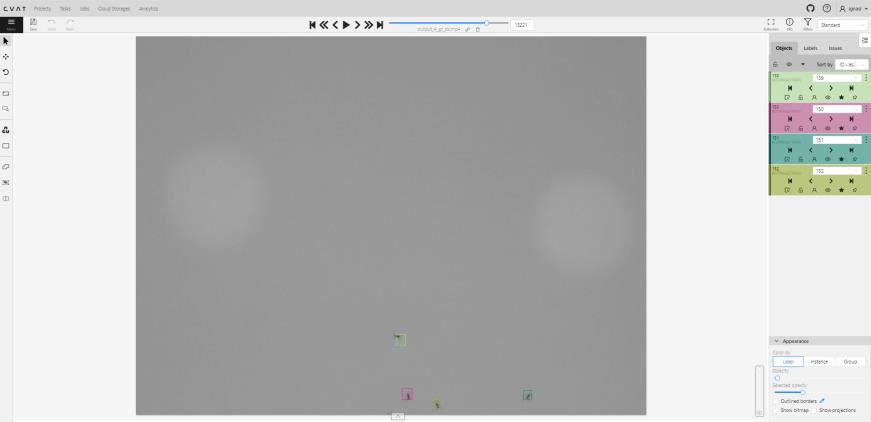
\includegraphics[width=0.7\linewidth]{figures/05_methodology/CVAT.png}
    \caption[CVAT interface]{\footnotesize{A screenshot of the CVAT interface.}}
    \label{fig:CVAT}
\end{figure}

\subsubsection{Lonely Ant Frame Segmentation}

{
    In the process of generating video segment annotations from the collection of videos for appearance training, 
    a text file is filled manually with the previously listed specifications. 
    To speed up the process, a command that write the frame number on each frame using the ffmpeg tool is employed, as illustrated in Listing \ref{lst:frame_num_video}:
}

\begin{footnotesize}
    \begin{bashcode}[float=!h, label={lst:frame_num_video}, language=bash, caption={Command to write the frame number on each frame}]
        ffmpeg -i input.mp4 -vf "drawtext=fontfile=Arial.ttf: text=%{n}: fontsize=24: x=(w-tw)/2: y=h-(2*lh): fontcolor=white@0.5: box=1:boxcolor=0x00000099@0.3" -y input_frame_num.mp4
    \end{bashcode}
\end{footnotesize}
\FloatBarrier

{
    This approach reduces the time required for annotation to approximately 15 minutes for every hour of video footage. 
    Note that a video can be played at an accelerated speed, and this annotations only require pausing the video.
}

{
    Moreover, when dealing with sequences involving only one ant per frame and employing a high-performance detector, 
    this method becomes analogous to annotating in the MOT Challenge format. 
    By utilizing \textbf{detection by tracking}, the detector can effectively allow the low-confidence detections\footnote{This improves the detection recall, recall is a metric that will be explained in the following subsection about metrics.} and utilize a tracker to eliminate false positives.
    Even if the detector does not eliminate all the false positives, 
    adhering to the strict criterion of one ant per frame enables the initial exclusion of frames featuring multiple ants, 
    which can subsequently be interpolated as required.
}

\subsubsection{Purging by Deletion}

{
    A reliable object detector relies on a clean object detection dataset. 
    Given the impracticality on annotating with \ac{CVAT}, a different approach to create a object detection dataset was designed.
    This process utilized the script previously explained for generating a cropped (or uncropped) YOLO dataset, as illustrated in Figure \ref{fig:yolo crop}.
    To accomplish this, two additional scripts were developed.
}

{
    The initial step involves generating the object detection dataset using the YOLO dataset script. 
    The image filenames are assigned based on the frame IDs 
    (if no cropping was applied, it can be easily transformed into the MOT format).
}

{
    Next, the second script comes into play, which annotates the images and saves them in a new folder. 
    In cases where only one detection exists, a crop is retained, as it simplifies the process of assessing its accuracy via a file explorer. 
}

{
    Subsequently, annotators are tasked with deleting the invalid images from this folder.
}

{
    In the final step, a script is employed to construct a new dataset by copying only the remaining images. 
    This results in an object detection dataset where only a fraction of the frames are preserved, 
    typically less than half of the images prove to be valid.
}

{
    As an example, 50 seconds (equivalent to 750 frames) are transformed into 13,000 crops, 
    equivalent to a duration of approximately 14 minutes and 27 seconds. 
    The annotation process for this sequence typically takes around 4 hours to complete.
}

\subsubsection{Cleaning by Crop Deletion}

{
    While discarding images containing errors is an acceptable practice for object detection datasets, the aim is often to maximize available data. 
    To address this, we implemented another set of scripts, similar to the ones described previously.
}

{
    In this scenario, the data is initially in MOT format both at the beginning and the end of the process. 
    The first script is designed to store cropped images alongside their corresponding frame IDs and line numbers.  
    This script can source data from either one or two models. 
    In cases involving two models, it combines their outputs and attempts to identify true positives (which can be reviewed more swiftly), false positives, and false negatives.  
}

{
    The second script generates a MOT format file containing only the remaining lines, meaning that annotations for frames are corrected rather than deleted.
}

{
    In this case, cleaning 1 hour of video containing a single ant (equivalent to 54,000 frames) can be accomplished in roughly 6 hours. 
    This process was applied to 9 out of the 12 individual ant videos.
}

\needspace{0.2\textheight}

\subsubsection{Labeling strategies summary}

{
    The following table shows the speed of each strategy:
}

\begin{table}[H]
    \centering
    \caption[Labeling strategies speed]{ \footnotesize Labeling strategies speed }
    \label{tab:labeling speed}

    \begin{tabularx}{0.7\textwidth}{
        @{\hspace{0.05\textwidth}}
        >{\raggedright\arraybackslash}X
        >{\raggedleft\arraybackslash}X
        @{\hspace{0.05\textwidth}}
    }
        \toprule
        \textbf{Strategy} & \textbf{Speed} \\
        \midrule
        \midrule
        CVAT & 0.2 fps \\
        Lonely ant frames & 60 fps \\
        Purging by deletion & 0.9 fps \\
        Cleaning by deletion & 2.5 fps \\
        \bottomrule
    \end{tabularx}
\end{table}
